\chapter{Deep Wavelet Super Resolution}


Pierwszy z omawianych algorytmów adresuje problem super-rozdzielczości obrazów przy użyciu transformacji falkowej i głębokiej sieci neuronowej. Algorytm został opracowany przez: Tiantong Guo, Hojjat Seyed Mousavi, Tiep Huu Vu, Vishal Monga, dla: School of Electrical Engineering and Computer Science, The Pennsylvania State University, State College, PA, 16803 \cite{guo2017deep}.
Ta głęboka sieć neuronowa skupia się na rekonstrukcji różnic pomiędzy obrazkiem wejściowym o niskiej rozdzielczości (LR - Low Res), a obrazkiem wysokiej rozdzielczości (HR - High Res). W tej pracy badane są zalety wykorzystywania danych domeny transformacji falkowej w zadaniu SR, zwłaszcza w celu uchwycenia większej ilości informacji strukturalnych w obrazach aby uniknąć artefaktów. 

Rezydualne sieci neuronowe korzystają z nieliczności danych wejściowych i wyjściowych oraz faktu, że uczenie sieci z nielicznymi aktywacjami jest znacznie łatwiejsze i bardziej niezawodne. 
To pozwala na wykorzystanie przestrzennych współczynników falkowych, które zazwyczaj są rzadkie. Co ważniejsze, wykorzystanie różnic współczynników falkowych jako par danych treningowych dodatkowo zwiększa rzadkość danych treningowych, co skutkuje bardziej efektywnym uczeniem. Innymi słowy, użycie współczynników falkowych sprzyja rzadkości aktywacji w warstwach środkowych, a także w warstwie wyjściowej.

\begin{figure}[ht]
    \centering
    \begin{minipage}[t]{0.35\linewidth}
        
\includegraphics[width=\linewidth]{Rozdziały/02.Podstawy_teoretyczne/Obrazy/comic.png}
        \caption{Obraz wejściowy}
        \label{fig:image46}
    \end{minipage}
    \hspace{0.5cm}
    \begin{minipage}[t]{0.35\linewidth}
        
\includegraphics[width=\linewidth]{Rozdziały/02.Podstawy_teoretyczne/Obrazy/comic_DWSR_x4.png}
        \caption{Obraz powiększony algorytmem DWSR czterokrotnie}
        \label{fig:image47}
    \end{minipage}
\end{figure}

Dodatkowo transformacja falkowa dekomponuje obraz na wiele skal, co pozwala na wykorzystanie informacji z różnych skal w celu rekonstrukcji obrazu o wysokiej rozdzielczości. W przeciwieństwie do innych metod, które wykorzystują informacje z jednej skali, DWSR wykorzystuje informacje z wielu skal, co pozwala na lepsze odwzorowanie obrazu o wysokiej rozdzielczości.


\section{Architektura DWSR}

Na problem super-rozdzielczości mozemy spojrzeć jak na problem rekonstrukcji detali w obrazie wejściowym o niskiej rozdzielczości. Takie podejście świetnie współgra z dekompozycją transformacji falkowej. Jak widać na Rys \ref{fig:image48}, jeśli potraktujemy obraz wejściowy jako wyjście LL poziomu 2dDWT, przewidywanie podpasm HL, LH i HH 2dDWT da nam brakujące szczegóły obrazu LL. Następnie można użyć 2dIDWT, aby zebrać przewidywane szczegóły i wygenerować wyniki SR.


\begin{figure}[ht]
    \centering
    \begin{minipage}[t]{0.7\linewidth}
        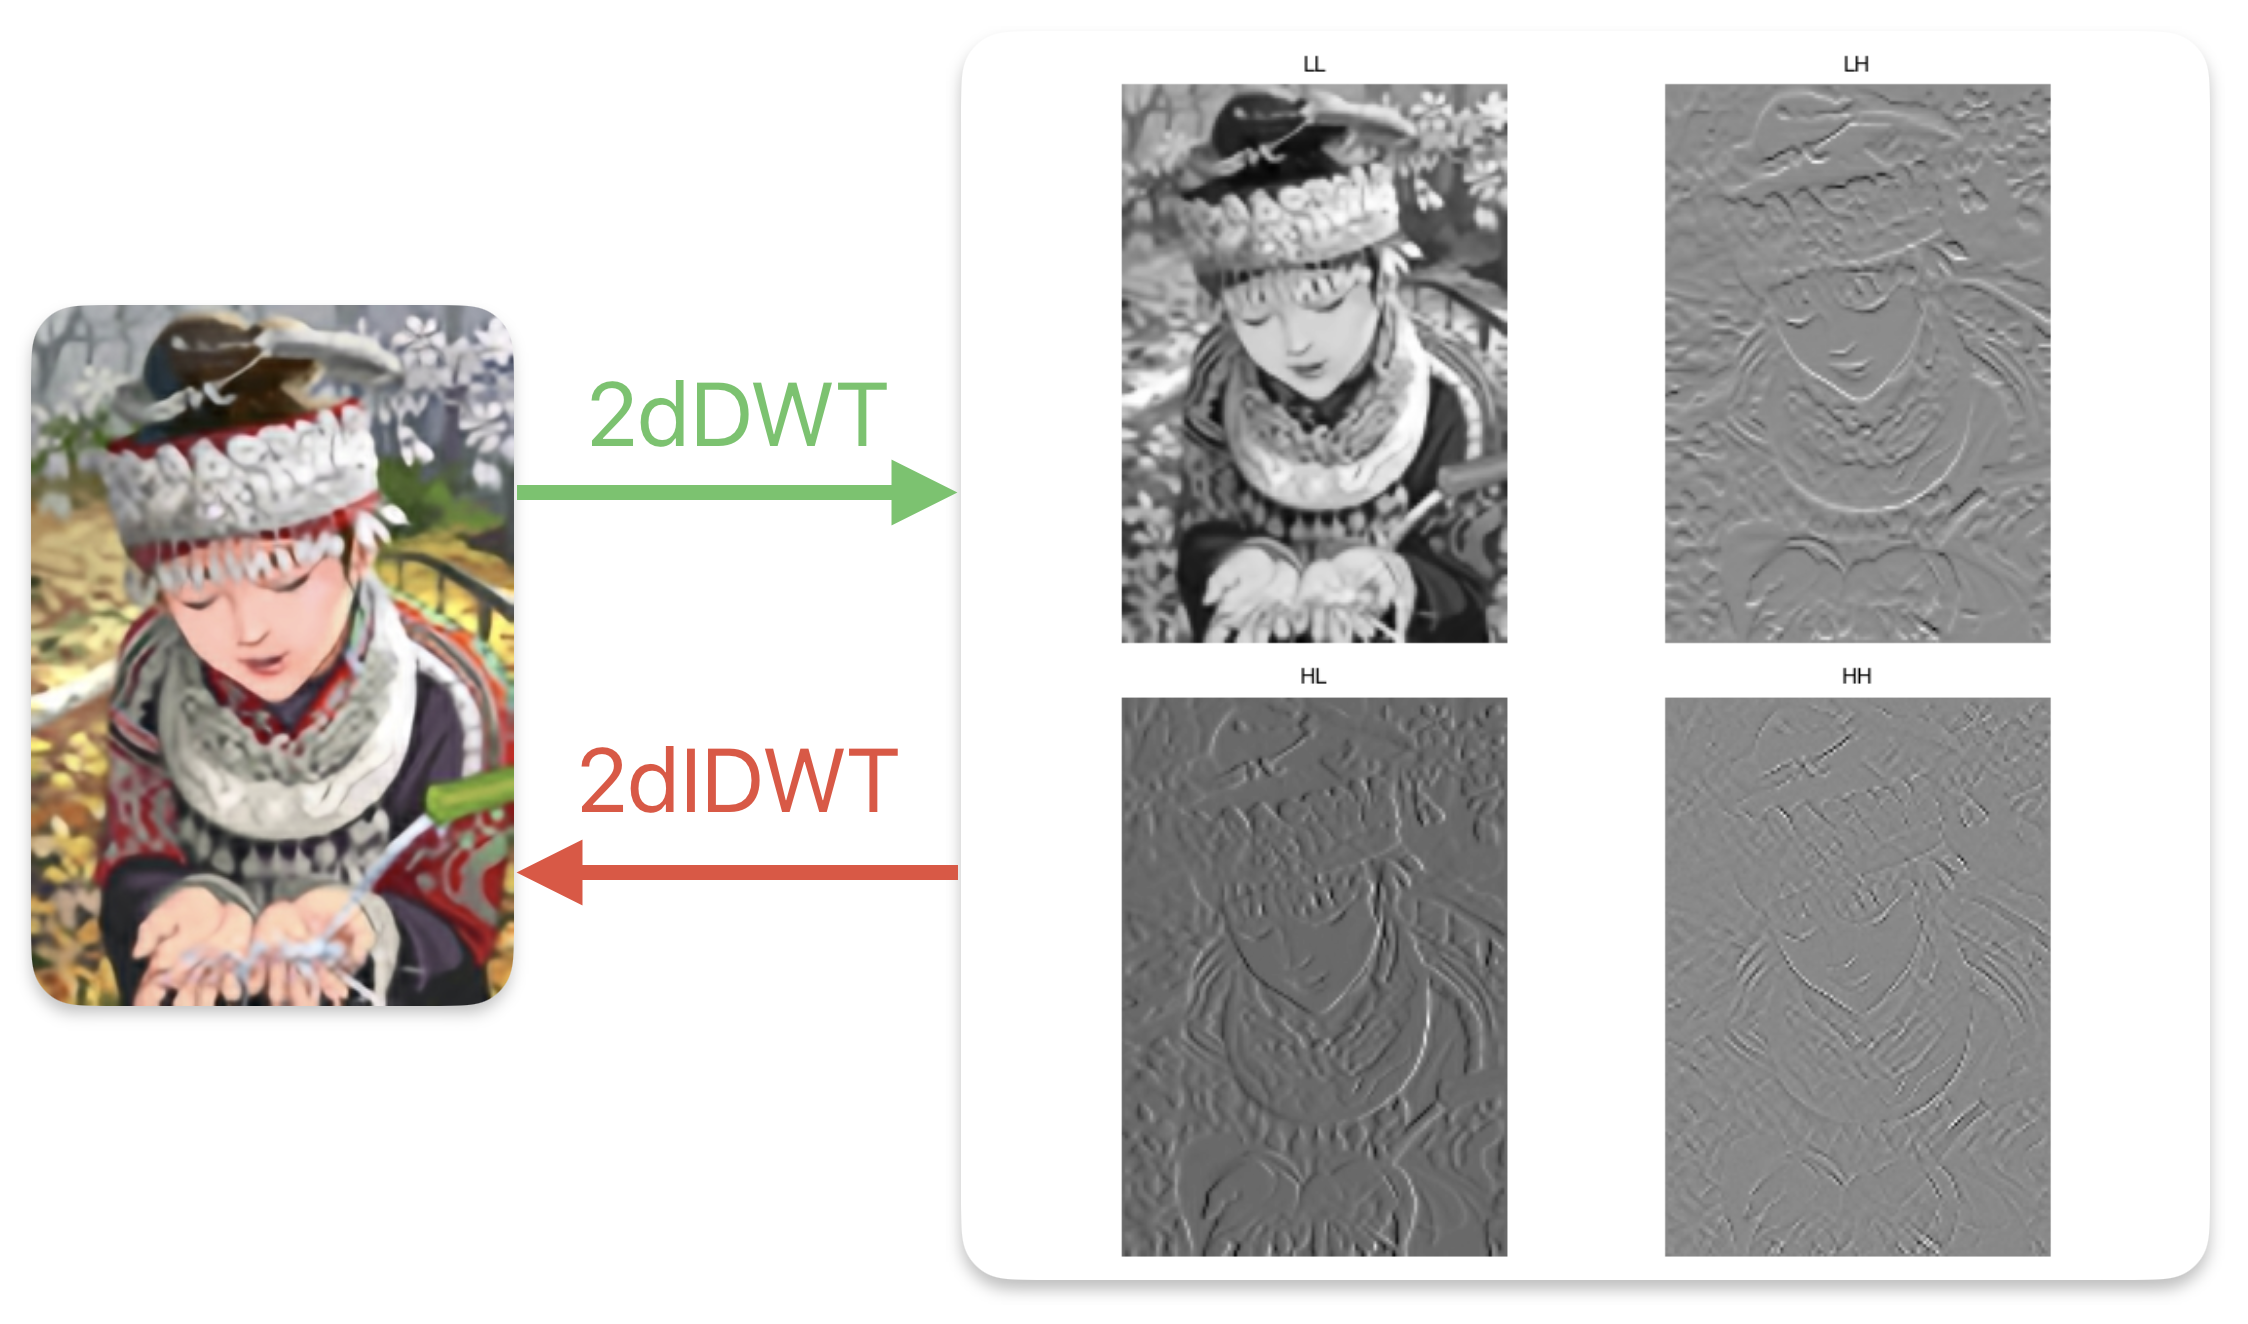
\includegraphics[width=\linewidth]{Rozdziały/03.DWSR/Obrazy/konstrukcja_2dDWT.png}  
        \caption{Proces dekompozycji Dyskretnej Transformacji Falkowej}
        \label{fig:image48}
    \end{minipage}
\end{figure}


Korzystając z falki Haar, współczynniki 2dDWT można zapisać jako:
\begin{equation*}
    \left\{\begin{array}{l}
    A=a+b+c+d \\
    B=a-b+c-d \\
    C=a+b-c-d \\
    D=a-b-c+d
    \end{array}\right.
\end{equation*}
gdzie: 
\begin{itemize}
    \item $A, B, C, D$ są pikselami zlokalizowanymi w siatce $2 \times  2$ w lewym górnym rogu obrazu HR,
    \item $a$ jest pikselem zlokalizowanym w lewym górnym rogu obrazu LL,
    \item $b$ jest pikselem zlokalizowanym w lewym górnym rogu obrazu HL,
    \item $c$ jest pikselem zlokalizowanym w lewym górnym rogu obrazu LH,
    \item $d$ jest pikselem zlokalizowanym w lewym górnym rogu obrazu HH.
\end{itemize}

Dlatego przy pomocy transformacji falkowej, problem SR staje się predykcją współczynników falkowych.


\section{Kluczowe cechy i innowacje}


Dyskusja na temat głównych innowacyjnych rozwiązań zastosowanych w DWSR i ich wpływu na efektywność metody.


\section{Proces treningu i implementacji}


Wyjaśnienie procedur związanych z treningiem DWSR, z uwzględnieniem specyfikacji danych, procesu uczenia i kwestii implementacji.


\section{Przykłady zastosowań i rezultaty}


Ilustracja praktycznych zastosowań DWSR oraz ocena i interpretacja osiągniętych dzięki niemu wyników.
